\documentclass[UTF8]{ctexart}
\usepackage{geometry}
\usepackage{amsmath}
\usepackage{graphicx} %插入图片的宏包
\usepackage{float} %设置图片浮动位置的宏包
\geometry{a4paper,scale=0.8}
\sectionfont{\bfseries\Large\raggedright}

\title{machine learning笔记}
\author{徐世桐}
\date{}
\begin{document}
\maketitle

% ----------------------------------------------------------------------
% |                              基础定义                               |
% ----------------------------------------------------------------------
\section{基础定义}
\noindent \textbf{二元分类}:输出分类个数为2\\
\textbf{多元分类}:输出分类个数不限

  $one-versus-the-rest$ OvR:计算属于每一分类的可能性,取可能性最大的分类为输出分类

  $one-versus-one$ OvO:对所有分类两两使用二元分类,每一分类器训练只需一部分数据\\
\textbf{multilabel多标签分类}:目标检测,对一图像中的物体加label\\
\textbf{multioutput多类分类}:多标签分类,每一标签可包含多种信息\\
\textbf{learning schedule}:根据迭代次数更新学习率\\
\textbf{early stopping}:提早结束训练

  对于每一epoch,当验证集MSE值增高时,证明开始overfit,停止训练

  即在epoch-error图中泛化误差最低时停止训练\\
\textbf{在训练中使用正则化代价函数,训练结束后测试中代价函数不使用正则化项}

% ----------------------------------------------------------------------
% |                              数学计算                               |
% ----------------------------------------------------------------------
\section{数学计算}
\noindent \textbf{MSE} = $\frac{1}{m}\sum_{i=1}^{m}(x^{(i)} - \bar{x} )^2$\\
\textbf{rigid regression}:回归方法,$J(\theta) = MSE(\theta) + \frac{\alpha}{2}\sum_{i}\theta_i^2$

  降低所有权重值\\
\textbf{lasso regression}:回归方法,$J(\theta) = MSE(\theta) + \alpha \sum_i |\theta_i|$

  降低不重要的权重值\\
\textbf{elastic net}:回归方法,$J(\theta) = MSE(\theta) + \gamma\alpha \sum_i |\theta_i| + (1-\gamma)\frac{\alpha}{2}\sum_{i}\theta_i^2$\\
\textbf{Normal Equation}:$\hat{\theta} = (X^TX)^{-1}X^Ty$

  直接得到权重$\hat{\theta}$,适用于仅有一个输出值的模型

  $X$为 (批量大小, 参数个数)输入矩阵,$y$为(批量大小, )向量
  
  当$X^TX$无逆矩阵时,用psudo inverse$\hat{\theta} = X^+y$\\
\textbf{pseudo inverse}:

  对矩阵$X=USV^T$,pseudo inverse $X^+=VS^+U^T$。$S^+$求法:

  \quad 1.对所有$S$元素,接近0的值赋为0

  \quad 2.对所有非零元素取倒数

  \quad 3.取矩阵转置,得到$S^+$\\
\textbf{log loss}:代价函数

  $J(\theta) = -\frac{1}{|B|}\sum_{i=1}^{|B|}[y^{(i)}log(\hat{p}^{(i)}) + (1-y^{(i)})log(1-\hat{p}^{(i)})]$

  标签值$y^{(i)}$为离散1/0值,计算值$\hat{p}^{(i)} \in [0,1]$

  微分:** 推导 **
  
  \quad $\frac{d J(\theta)}{d \theta_j} = \frac{1}{|B|}\sum_{i=1}^{|B|}(\hat{p}^{(i)} - y^{(i)}) x_j^{(i)}$\\
\textbf{Hinge loss}:代价函数

  $HingeLoss(y, \hat{y}) = max(0, 1-y*\hat{y})$

  应用于SVM,$y \in \{0, 1\}$,$\hat{y} \in \mathbb{R} $
  
  代表当预测值$\hat{y}$和y同号,$\hat{y} \geq 1$,则预测值和标签匹配,代价$=0$。否则$y*\hat{y} < 1$。代价值上升\\
\textbf{Gaussian Radial Basis Function RBF}:一种similarity function

  $\phi_{\gamma}(x, l) = exp(-\gamma||x-l||^2)$

  \quad $l$为landmark,即$\phi_{\gamma}$由一样本$x_i$和一landmark的距离得来\\
\textbf{Lagrange multipliers method拉格朗日乘数法}

  将\ 有前提的多项式求最值\ 问题转化为\ 无前提多项式最值问题

  定义:

  \quad 对输入向量$W$,$g(W) \geq 0$为constrain。目标为在满足$g(W) \geq 0$的前提下取$f(W)$最值

  \quad Lagrange function $\mathcal{L} (W, \alpha) = f(W) - \alpha(g(W))$

  \quad \quad $\alpha$为需要求解的变量之一,参与最终计算$W$的值。

  \quad \quad 当有多个constrain $g^{(i)}(W)$时,$\vec{\alpha}$为向量,求偏导对每一$\vec{\alpha}^{(i)}$求导

  \quad \quad 只有当$\alpha \geq 0$ 或每一$\vec{\alpha}^{(i)} \geq 0$,结果才有效

  \quad \quad $\vec{\alpha}^{(i)} = 0$代表对应的constrain $g^{(i)}(W)$为一个support vector

  计算:
  
  \quad 对每一$W$的元素\ 和\ $\alpha$取偏导,即向量
  $\begin{bmatrix}
    \frac{d \mathcal{L}(W, \alpha)}{d w_1}  \\
    \frac{d \mathcal{L}(W, \alpha)}{d w_n} \\
    ... \\
    \frac{d \mathcal{L}(W, \alpha)}{d w_n} \\
    \frac{d \mathcal{L}(W, \alpha)}{d \alpha}
  \end{bmatrix}$,计算向量$=\vec{0} $时的$W$, $\alpha$取值




% ----------------------------------------------------------------------
% |                             分类模型                                |
% ----------------------------------------------------------------------
\section{分类模型}
\noindent \textbf{logistic regression}:

  判断输入符合每一输出类别的可能性,

  前向计算:
  
  \quad 1.$\hat{p} = \sigma(\theta^Tx + b)$

  \quad 2.$\hat{y} = 1\space (if \hat{p} \geq 0.5)$

  \quad \quad \quad $= 0\space (if \hat{p} < 0.5)$

  代价函数为log loss\\
\textbf{SVM}

  找到分界,分离多种数据

  support vector: 最靠近分界线的样本

  hard margin classification硬性分类:限制数据必须被分界隔开,同一类数据不可同时出现在分界2端

  soft margin classification:与硬性分类相反,避免被outlier离群值影响

  前向计算:$\hat{p} = f(x_1, x_2,...)$,其余同logistic regression

  \quad 区别:$f$可为polynomial,非线性函数。可使用kernel trick

  线性分类训练:$\hat{p} = W^Tx + b$,$W$ 为参数\textbf{向量}

  \quad \textbf{硬性分类}:

  \quad \quad $||W||_2$代表线性函数斜率

  \quad \quad 最小化$\frac{1}{2}W^TW$,使得分界平面的斜率最小,最大化分界线和两种数据的距离

  \quad \quad 前提:对每一样本$i$, $1.y^{(i)}\hat{p}^{(i)} \geq 1$,即标签和计算结果相同

  \quad \quad 求解:1.直接解以上带前提的不等式

  \quad \quad \quad '当样本数高于参数数量时使用,由于dual form的复杂度为$O(|S|^2)$ - $O(|S|^3)$,直接解复杂度为$O(|S|)$'
  
  \quad \quad 2.使用拉格朗日乘数法得到dual form,其中$\vec{\alpha}$为向量。$\textbf{x}^{(i)}$为第i样本的特征值向量$\mathcal{L} = \frac{1}{2}W^TW - \sum_{i=1}^{|B|}\vec{\alpha}^{(i)}(y^{(i)}\hat{p}^{(i)} - 1)$

  \quad \quad \quad 使偏导向量为$\vec{0} $,得到$2.W = \sum_{i=1}^{m}\vec{\alpha}_iy^{(i)}\textbf{x}^{(i)}$, $3.\sum_{i=1}^{m}\vec{\alpha}_iy^{(i)}=0$

  \quad \quad \quad 带入得$\mathcal{L} (W, \vec{\alpha}) = \frac{1}{2}\sum_{i=1}^{|B|}\sum_{j=1}^{|B|}\vec{\alpha}_i\vec{\alpha}_jy^{(i)}y^{(j)}\textbf{x}^{(i)^T}\textbf{x}^{(j)} - \sum_{i=1}^{|B|}\vec{\alpha}^{(i)}$
  
  \quad \quad \quad \quad $=\frac{1}{2}\vec{\alpha}^T (\textbf{x} * y)(\textbf{x} * y)^T \vec{\alpha} - \sum_{i=1}^{|B|}\vec{\alpha}^{(i)}$

  \quad \quad \quad \quad 其中$(\textbf{x} * y)$为广播乘法\ 将训练集矩阵每一样本乘以对应标签值,$y$为标签列向量

  \quad \quad \quad 使用QP solver得到使$\mathcal{L} (W, \vec{\alpha})$最小,$\vec{a}^{(i)} \geq 0$的向量$\vec{\alpha}$

  \quad \quad \quad 解$W$:由$\vec{\alpha}$带入2.式计算,$\vec{\alpha}$已被clamp,见经验2.

  \quad \quad \quad 解$b$:由于所有support vector $\textbf{x}^{(i)}$ 满足1.式,则对所有support vector计算$b$取平均值

  \quad \quad \quad \quad $b = E_{a^{(i)} \geq 0}(y^{(i)}-W^T\textbf{x}^{(i)})$

  \quad \quad 3.直接进行梯度下降,代价函数$J(W, b) = \frac{1}{2}W^TW + const \sum_i HingeLoss(y^{(i)}, \hat{p}^{(i)})$
  
  \quad \textbf{软性分类}:

  \quad \quad 最小化$\frac{1}{2}W^TW + C\sum_{i=1}^{|B|}\zeta_i $

  \quad \quad \quad $\zeta_i$定义第$i$样本被忽视为误差样本的可能性,$C$定义忽视率相对斜率的权重

  \quad \quad 前提:对每一样本$i$,$y^{(i)}\hat{p}^{(i)} \geq 1 - \zeta^{(i)}$

  非线性分类方法:

  \textbf{- 使用polynomial做$f$}

  \quad 必须使用拉格朗日乘数法求解,目的为\textbf{对$\phi(x)$得到线性权重和偏差},求解使用dual form,其中包含$\phi(a)^T \cdot \phi(b)$项即可使用kernel method

  \quad 权重$W$公式不再适用,由于结果不为线性

  \quad 偏差$b = \sum_{\vec{\alpha}^{(i)} \geq 0} y^{(i)} - \sum_{\vec{\alpha}^{(j)} \geq 0} \vec{\alpha}^{(i)} * y^{(j)} * K(\textbf{x}^{(i)}, \textbf{x}^{(j)})$

  \textbf{- 使用similarity function}:
  
  \quad 选择多个landmark$\mathcal{L} = l_1, l_2, ..., l_n$,对每一样本$x_i$计算其和每一$l_j$的$\phi_{\gamma}$值$\phi_{\gamma}(x_i, l_j)$

  \quad 每个样本用新的向量$x_i' = \begin{bmatrix}
    \phi_{\gamma}(x_i, l_1) \\
    \phi_{\gamma}(x_i, l_2) \\
    ... \\
    \phi_{\gamma}(x_i, l_n)
  \end{bmatrix}$表示。新的向量组成训练集,进行SVM训练

  \textbf{kernel}:

  \quad 定义:能够从输入向量$a$,$b$,不通过计算$\phi(a), \phi(b)$直接得到点乘结果$\langle \phi (a), \phi (b)\rangle $的函数

  \quad 例:** 是否通过取linear 为phi得到kernel 函数 **

  \quad \quad linear: $f(a, b) = a^Tb$

  \quad \quad polynomial: $f(a, b) = (\gamma a^Tb+r)^d$

  \quad \quad \quad poly的$\phi(x)$为对向量x每一元素进行poly运算,结果向量元素数不变

  \quad \quad Gaussian RBF: $f(a, b) = exp(-\gamma ||a-b||^2)$

  \quad \quad Sigmoid: $f(a, b) = tanh(\gamma a^Tb + r)$

  \quad \textbf{经验总结}:

  \quad \quad 1.QP solver中需限定$\sum_{i=1}^{m}\vec{\alpha}_iy^{(i)}=0$,否则得出$\hat{\alpha}$不遵循此等式

  \quad \quad 2.当样本有重叠,仍可使用拉格朗日乘数法,异常样本被分入错误类别。

  \quad \quad \quad 此时$\vec{\alpha}$包含负值,对应的样本在计算权重\ 偏差时被忽略,即需clamp使$\vec{\alpha} \geq 0$

  \quad \quad \quad 若不进行clamp,得到的分界仅有略微差别,不会造成大幅误差。(在线性\ 非线性分类都有验证)

  \quad \quad 3.梯度下降直接得到最优$W, b$,无法通过梯度下降得到$\vec{\alpha}$ 由于梯度下降忽略限制条件

  \quad \quad 4.QP solver需要$(\textbf{x} * y)(\textbf{x} * y)^T$为positive definite,计算时加上对角矩阵$diag(\epsilon)$即可,$\epsilon$多取$10^{-4}$

  \quad \quad \quad 否则迭代解QP时出现KKT condition not met或positive definite条件不满足

  \quad \quad \quad 条件不满足时中断得到的$\vec{\alpha}$无法作为有效结果参与后续计算权重和偏差

  \quad \quad \quad 优先将此矩阵转为float64类型,否则需要$\epsilon$较大才能保证positive definite
  

% ----------------------------------------------------------------------
% |                              决策树                                 |
% ----------------------------------------------------------------------
\section{决策树}
\noindent 定义:

  节点$N_i$:

  \quad 节点条件:判断样本进入哪一子节点,叶节点没有节点条件
  
  \quad sample属性$S_i$:有多少样本\textbf{进入$N_i$节点},非满足$N_i$节点条件的样本个数

  \quad value属性$V_i = v_{i1}, ..., v_{in}$:$S_i$进入节点的样本中$v_i$个属于第$i$分类

  \quad gini属性$G_i$:数据混杂度,$G_i = 1-\sum_{j=1}^{n}(\frac{v_{ij}}{S_i})^2$
  
  \quad 子节点仅有2个,对应节点条件为true/false的情况\\
分类方式:数据从根节点开始,根据节点条件传向对应子节点。直到到达叶节点。叶节点中$V$属性中最大项即数据分类\\
\textbf{CART algorithm创建决策树}:

  根节点初始化为叶节点,没有节点条件
  
  对每一叶节点$S_i$选取一特征$k$,一特征门槛$t_k$,将样本集分为2组$S_{true}, S_{false}$。
  
  \quad 选取$(k, t_k)$方式:使代价函数$J(k, t_k) = \frac{S_{true}}{S_i}G_{true} + \frac{S_{false}}{S_i}G_{false}$最小

  直到决策树层数达到固定上限,或对所有分组条件$(k, t_k)$,$J(k, t_k) \geq G_i$\\
\textbf{使用决策树进行regression}

  \begin{figure}[H] %H为当前位置,!htb为忽略美学标准,htbp为浮动图形
    \centering %图片居中
    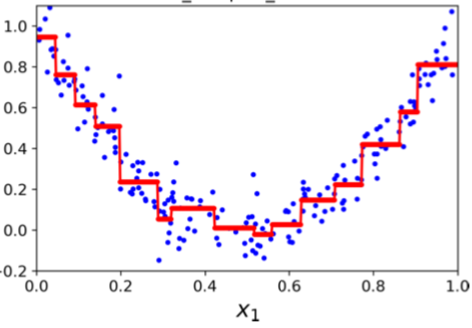
\includegraphics[width=0.3\textwidth]{note_images/deci_tree_regression.png} %插入图片,[]中设置图片大小,{}中是图片文件名
  \end{figure}

  输入样本,分类进不同值域

  更改:
  
  \quad 每一节点value值为一常数,为$S_i$样本的平均值。
  
  \quad 输出值为叶节点的value,非最大value对应的类别

  \quad $G_i$为$S_i$样本的方差$\frac{1}{S_i}\sum_{j=1}^{S_i}(x_i^{(j)} - \bar{x}_i)^2$

% ----------------------------------------------------------------------
% |                 ensemble learning random forest                    |
% ----------------------------------------------------------------------
\section{ensemble learning \& 随机森林}
\noindent \textbf{ensemble learning}:使用一组预测机制进行学习,预测机制可为不同算法\\
\textbf{random forest随机森林}:

  训练方法:随机选择$n$个训练子集$s_1, s_2, ..., s_n \in S$,训练$n$个决策树$t_1, ..., t_n$。
  
  前向计算:对$n$个树产生的$n$个分类结果,选取投票最多的一分类作为结果
  
  训练子集选取:bagging:子集可重复选取一样本,pasting:样本不重复
  
  \quad out-off-bag oob 样本:当使用bagging选取时,平均只有$1-e^{-1}$样本被选择,余下样本被称为oob样本

  优化:

  \quad random patches随机贴片:对特征和训练集同时取子集进行训练
  
  \quad random subspace随机子空间:对特征取子集,对整个总训练集进行训练
  
  \quad extra-trees极度随机森林:'使用随机$t_k$而不使用最小化数据混杂度的$t_k$'
  
  \quad $k$feature importance特征重要性:对所有取$k$为判断条件的节点$N_i$,计算加权平均值$\sum_i(S_i$imprity降低百分比$)$
  
  \quad (hypothesis) boosting:合并多个预测机制据结果的方法
  
  \quad \quad AdaBoost:串联预测机制,对上一预测机制遗漏的样本加更高权重,进行训练

  \quad \quad gradient boosting


% ----------------------------------------------------------------------
% |                     dimentionality reduction                       |
% ----------------------------------------------------------------------
\section{维度下降}
\noindent 根据manifold assumption,高维空间中训练集参数点稀疏。则将数据压缩到低维\\
\textbf{principle component analysis PCA}:

  对训练集参数矩阵取SVD$USV^T$

  取$V$中前$d$个向量$V' = [v_1, ..., v_d]$,新训练集$A_{compressed} = A_{origin}V'$
  
  从\ 新训练集\ 延展回\ 原训练集纬度:$A_{expand} = A_{compressed}V'^T$\\
\textbf{Incremental PCA}:无需整个训练集存在内存中即可进行SVD\\
\textbf{kernel PCA}:**\\
\textbf{local linear Embedding LLE}:
  
  对每一样本$x^{(i)}$寻找$k$个相邻样本\ 相邻样本index的集合称$C_{x^{(i)}}$
  
  构建$(|S|, |S|)$矩阵$W$:
  
  \quad 每一行向量$[W_{i1}, ..., W_{i|S|}]$满足$x^{(i)} - \sum_{j \in C_{x^{(i)}}} W_{ij}x^{(j)}$
  
  \quad 每一行向量$W_i$求和为1:$\sum_{i=1}^{|S|}W_i = 1$

  由$W$创建新训练集:

  \quad 令$z^{(i)}$为$x^{(i)}$在低维的投影

  \quad 使所有$z^{(i)}$满足最小化$(z^{(i)} - \sum_{j=1}^{|B|}w_{ij}z^{(j)})^2$

% ----------------------------------------------------------------------
% |                             无监督学习                               |
% ----------------------------------------------------------------------
\section{无监督学习}
\noindent \textbf{clustering}\\
\textbf{K-mean}:

  将数据分为k个cluster,每个cluster有中心点称centroid
  
  算法:
  
  \quad 1.初始化随机选择k个样本位置做centroid

  \quad 2.分配样本:每个样本分入距离最近的centroid的cluster

  \quad 3.更新centroid:新centroid为cluster中样本坐标平均值。
  
  \quad 重复第2.3.步,直至centroid不再移动

  优化:
  
  \quad 多次随机初始化centroid,选择其中inertia最小的centroid取法进行训练

  \quad \quad interia = $\frac{1}{|S|}\sum_x (C_x - x)^2$。

  \quad \quad \quad $C_x$为样本x距离最近的centroid

  \quad k-mean++初始化centroid:

  \quad \quad 1.随机选择1个样本做centroid

  \quad \quad 2.剩余每一样本$x^{(i)}$有$\frac{D(x^{(i)})}{\sum_{j=1}^{|S|} D(x^{(j)})}$几率被选做新centroid

  \quad \quad \quad $D(x^{(i)})$为样本$x^{(i)}$距离最近的centroid的距离

  \quad \quad 3.重复2.步直至得到k个centroid

  \quad (在尝试多种cluster训练后)选择cluster数量k:

  \quad \quad sihouette score:所有样本的sihouette coefficient的均值

  \quad \quad \quad 一样本$x^{(i)}$的sihouette coefficient:$\frac{b-a}{max(a, b)}$

  \quad \quad \quad \quad $a$为$x^{(i)}$到同一cluster内所有样本的平均距离
  
  \quad \quad \quad \quad $b = min(E_{x^{(j)} \in other \space cluster}(D(x^{(i)} - x^{(j)})))$

  \quad \quad \quad sihouette score$\in [-1, 1]$,偏向取score高的cluster数

  使用k-mean进行数据预处理:

  \quad 将数据首先进行k-mean分类,将每一样本替换为\ 样本到最近的centroid距离,传入另一模型进行学习

  \quad 用于半无监督学习:将数据进行k-mean分类,从每一cluster选取离centroid最近的样本,产生大小为k的训练集。则只需得到k个样本的标签即可进行训练\\
\textbf{DBSCAN}

  适用于一cluster内样本密度较高的训练集

  算法:

  \quad 1.对每一样本$x_i$计算集合$S_{i\varepsilon}$,称$\varepsilon -neighbourhood$,包含所有距离在$\varepsilon $内的其他样本

  \quad \quad $|S_{i\varepsilon}| > $超参数$s_{min}$\ 的样本称core instance

  \quad 2.所有属于同一$S_{i\varepsilon }$的样本判为属于同一cluster,当一样本$x_i$同时存在样本$x_i, x_j$的$\varepsilon -neighbourhood$中时,合并$S_{i\varepsilon }, S_{j\varepsilon }$。

  \quad 3.没有被分配进任何$S_{i\varepsilon }$的样本判为异常值\\
\textbf{Gaussian Mixtures}

  \textbf{GM Model}:假设所有样本都由多个正态分部产生


% ----------------------------------------------------------------------
% |                              对抗网络                                |
% ----------------------------------------------------------------------
\section{GAN对抗网络}
\noindent \textbf{基本结构}:

  generator:得到正则噪声,生成伪数据。
  
  discriminator,从实际数据集或generator得到数据判断真伪(是否来自实际数据集)。

  一次训练:

  \quad 1.discriminator从数据集得到一批量真实数据\ 和\ 一批量伪数据。使用二元交叉熵损失函数训练

  \quad \quad 目标为:对伪数据输出0\ 真数据1

  \quad 2.generator生成图像
  
  \quad \quad 目标为生成discriminator输出为1的数据\\
\textbf{Deep Convolutional GAN}


% ----------------------------------------------------------------------
% |                             RL强化学习                               |
% ----------------------------------------------------------------------
\section{RL强化学习}
\noindent \textbf{基本定义}

  程序在 environment环境中根据观测得到的 state状态,选择 action行为,得到reward反馈

  模型整体符号定义<A, S, R, P>

  \quad Action space $A$
  
  \quad State space $S$
  
  \quad Reward $R$: $\sum$ × $A$ × $S$ → $R$
  
  \quad Transition $P$: $\sum$ × $A$ → $S$

  第$i$决策的符号定义:

  \quad $a_i \in A$ 采取的行为

  \quad $r_i \in R$ 得到的reward,每一行为可以立即得到反馈值
  
  exploring探索:模型尝试新行为
  
  exploiting利用:模型使用已知高反馈行为\\
\textbf{policy}

  根据观测选择$a_i$的算法

  stochastic policy:policy中有随机性

  \quad 随机性提高模型 explore新行为

  generic algorithm:遗传算法

  policy gradients:对参数求导,更新参数\\
\textbf{credit assignment}:

  对每一决策分配discounted reward,代表此决策对随后几次决策的反馈值影响

  定义:

  \quad $l$ 此次试验一共包含的决策数

  计算:

  \quad 第$l-1$决策有决策有discounted reward:$dr_i = r_i$
  
  \quad 第$i$决策有discounted reward:$dr_i = r_i + \gamma dr_{i+1}$
  
  \quad 正则化:对所有实验中每一次决策$r_i$取整体平均值,方差,求标准化\\
\textbf{neural network policy}

  \textbf{前向传播}:使用神经网络得到行为可能性,根据可能性选择行为。属于generic gradient policy

  \textbf{迭代}:

  \quad 定义:一次决策

  \quad \quad 1.从policy得到行为可能性

  \quad \quad 2.代价函数根据\ 采取的行为\ 和\ \textbf{采取的}行为可能性\ 计算代价值

  \quad \quad 3.根据代价函数求斜率,斜率使神经网络输出可能性更偏向采取的行为。\textbf{但不立即使用斜率}

  \quad 1.随机初始化1次模型,对$n$个随机初始化环境进行试验,每一试验中包含多个决策
  
  \quad \quad 每一环境得到决策数不一定相同,取决于试验中进行的决策次数

  \quad 2.对每一决策求discounted reward
  
  \quad 3.对每一参数,斜率为$n$次训练中所有决策\ 对\ 此参数的斜率\ 的加权平均值。权重为discounted reward

  \quad 4.使用权重更新参数值\\
\textbf{Markov Decison Process MPD}

  每一状态$s_i$有可执行的行为集合$A_{s_i} \subseteq A$。不同状态行为集合可有交集

  行为$a_{ij} \in A_{s_i}$代表状态$s_i$执行行为$a_j$。执行$a_{ij}$后有$p_{a_{ij}, s_k}$几率到达状态$s_k$

  optimal state value $V^*(s_i)$:
  
  \quad 模型到达状态$s_i$后1.选择最理想的$a_{ij}$能得到的discounted reward总和

  \quad $V^*(s_i) = max_j \sum_s [p_{a_{ij}, s_k} (R(s_i, a_{ij}, s_j) + \gamma \cdot V^*(s_j))]$
  
  Q-value iteration algorithm:

  \quad 得到\ 从$s_i$选择$a_{ij}$后期望的discounted reward值

  \quad 迭代:$Q_{n+1}(s_i, a_{ij}) = \sum_j [p(a_{ij}, s_j) (R(s_i, a_{ij}, s_j) + \gamma \cdot max_{a_{jk}} (Q_n(s_k, a_{jk})))]$
  
  policy:状态为$s_i$时选取$a_{ij} = max_{a_{ij}} Q^*(s_i, a_{ij})$\\
\textbf{Temporal Difference Learning TD learing}

  在$p_{a_{ij}, s_j}$, $R$未知的情况下迭代得到$V(s_i)$\\
\textbf{Q-Learning}

  在$p_{a_{ij}, s_j}$, $R$未知的情况下迭代得$Q(s_i, a_{ij})$

  $Q_{n+1}(s_i, a_{ij}) = r'_i + \gamma \cdot max_k (Q_{n}(s_i, a_{jk}))$\\
\textbf{deep Q-networks DQNs}

  
% ----------------------------------------------------------------------
% |                              分析结果                                |
% ----------------------------------------------------------------------
\section{分析结果}
\noindent \textbf{confusion matrix困惑矩阵}:分析二元/多元分类
  
  $\begin{bmatrix}
    TN & FP \\
    FN & TP
  \end{bmatrix}$

  一行对应同一期望输出,一列对应同一计算输出

  $T/F$: 此位置的计算输出是否和预计输出一致

  $P/N$: 此位置的预计输出是否为真

  \textbf{precision} $= \frac{TP}{TP + FP}$

  \quad 即$P($计算结果匹配 $|$ 计算结果为正$)$

  \textbf{recall} = $\frac{TP}{TP + FN}$

  \quad 即$P($计算结果匹配 $|$ 预计结果为正$)$

  \textbf{$F_1$} $= \frac{2}{\frac{1}{precision} + \frac{1}{recall}}$ 
  
  \quad precision 和 recall的调和平均值
  
  \textbf{specificity} = $\frac{TN}{TN + FN}$\\
\textbf{ROC curve}:分析二元/多元分类

  \begin{figure}[H] %H为当前位置,!htb为忽略美学标准,htbp为浮动图形
    \centering %图片居中
    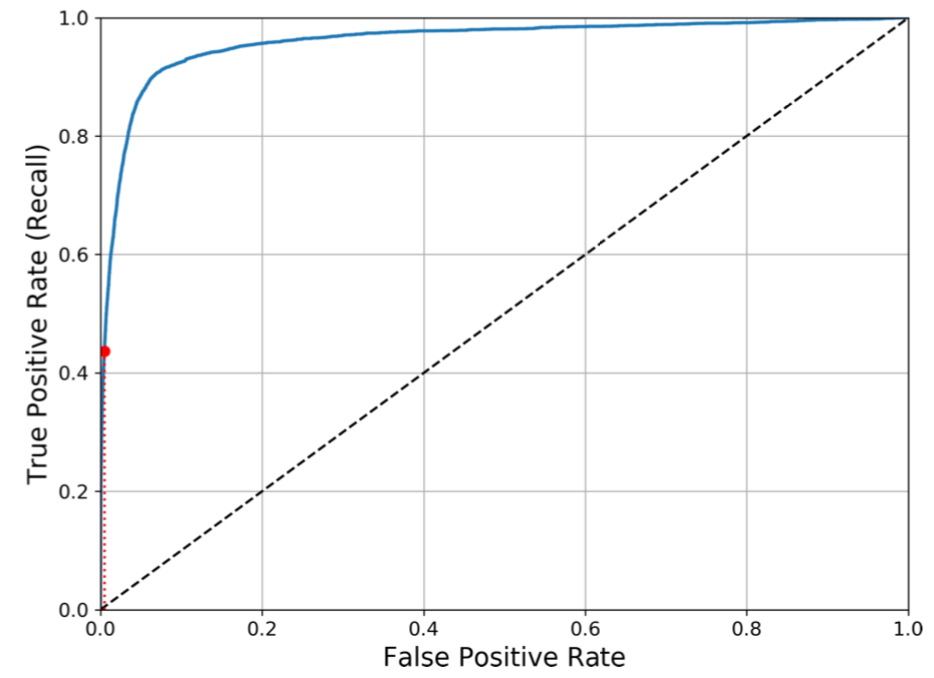
\includegraphics[width=0.3\textwidth]{note_images/ROC_curve.png} %插入图片,[]中设置图片大小,{}中是图片文件名
  \end{figure}

  y轴recall值,x轴false positive rate$FPR = \frac{FN}{FN + TN} = \frac{FN}{1-specificity}$

  期望的ROC curve为recall从0快速增长到1。并保持直到$FPR$为1。
  
  \quad 即期望曲线下方面积接近1\\
\textbf{learning curves}:观察模型是否有over underfit

  \begin{figure}[H] %H为当前位置,!htb为忽略美学标准,htbp为浮动图形
    \centering %图片居中
    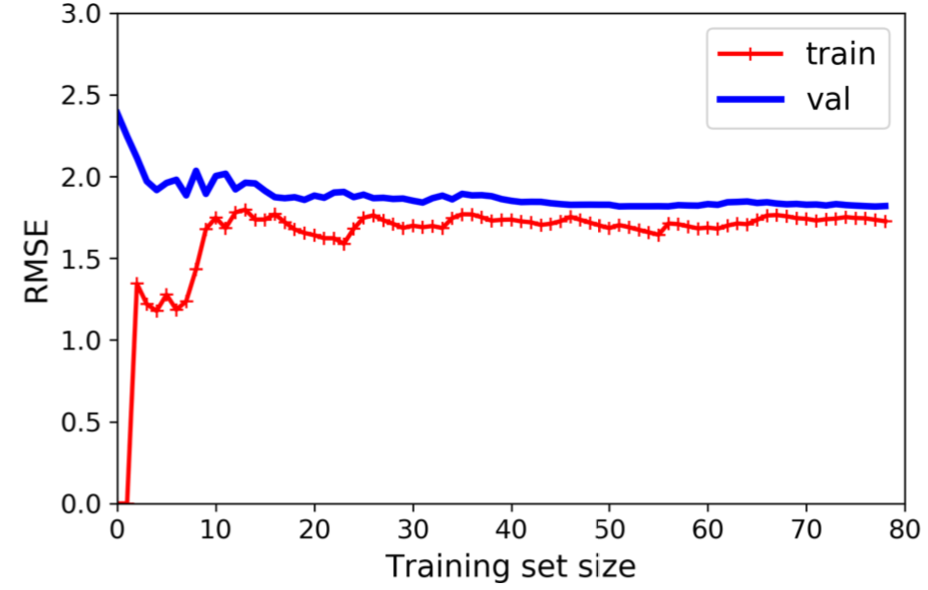
\includegraphics[width=0.3\textwidth]{note_images/learning_curve.png} %插入图片,[]中设置图片大小,{}中是图片文件名
  \end{figure}

  x轴为\textbf{一整次训练(包含多次epoch)使用的训练集大小},y轴为root MSE。

  画出训练集\ 测试集在使用不同训练集大小后的root MSE。

  分析:

  \quad 期望2曲线平缓值低且相近,

  \quad 当2曲线平缓值差值较大,测试集平缓值较低,则过拟合

  \quad 当2曲线平缓值较高,则欠拟合\\
\textbf{模型复杂度-error epoch-error}:

  \begin{figure}[H] %H为当前位置,!htb为忽略美学标准,htbp为浮动图形
    \centering %图片居中
    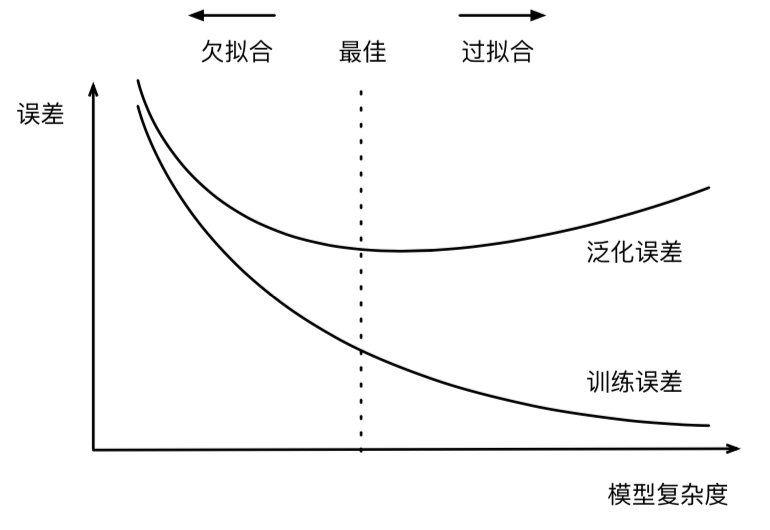
\includegraphics[width=0.3\textwidth]{note_images/epoch-complex-error.png} %插入图片,[]中设置图片大小,{}中是图片文件名
  \end{figure}

  2种图,形状类似,x轴内容不同\\

\end{document}
